\documentclass[11pt,letterpaper]{article}

\usepackage[hmargin=2.6cm,vmargin=2.5cm]{geometry}
\usepackage{algorithm}
\usepackage{algorithmic}
\usepackage{amsmath}
\usepackage{amsfonts}
\usepackage{enumerate}
\usepackage{graphicx}

\begin{document}
\title{CSMC 701 Project - Problem B}
\author{Rob Argue \and Tommy Pensyl}
\maketitle
\section{The Algorithm}
Consider in general we are matching $q$ queries of maximum length $m$ each, and $p$ references of maximum length $n$. Additionally, we are looking only for matches within an edit distance $k$.

\subsection{Dynamic Programming}
We started with a standard dynamic programming approach. We used the global alignment recurrence, with the initial column and row penalized as normal. Since we don't care about mismatches after the query, we take the final edit distance to be the smallest value in the last row (corresponding to the end of the query). This takes $O(mn)$ time and memory for each query-reference pair. 

We made two additional optimizations. First, we only keep track of two rows at a time, and second, we use the maximum edit distance $k$ to only consider cells which have a chance at being less than $k$. In the worse case it iterates over all cells within $k$ of the diagonal, taking $O(mk)$ time and $O(m)$ memory. In practice we may decrease the number of cells per row we examine as the algorithm finds more errors, and the algorithm will often cut off early (i.e. when the best score is already greater than $k$), so it does better.

Since we apply dynamic programming for each pair of query and reference, we would expect an overall worst-case runtime complexity of $O(pqmk)$. Using the test data provided, this method took over 10 hours to complete the matching.

\subsection{Letter Frequency Culling}
To reduce this time, we use a simple culling method based on letter frequency to eliminate some of the possible matches before ever starting the dynamic programming. Let $x$ be the minimum length of all queries and references. Then we calculate the letter frequencies for the first $x$ characters for each reference and query. Then, when comparing each query to a reference, we calculate the total of the absolute difference of each letter count between the two. We know each of the $k$ errors is either an insert, delete, or substitution. In any case, each error can increase this deviation by at most 2, so if the frequencies differ by more than $2k$, we know the edit distance must be more than $k$, and we can skip the dynamic programming altogether.

Additionally, we found it was helpful to apply this frequency-culling on prefixes of multiple lengths. For example instead of just looking at the first 185 characters, we may also look at the first 150 and the first 120. This further increases the amount of nonmatches that are culled early. (\emph{Ideally}, the prefix length should not be limited by the minimum-length query; this was just for simplicity of implementation.)

The letter frequencies are calculated just once for each query and reference, so this adds only an $O(q+p)$ term which is dominated by the other terms. The $O(qp)$ addition only involves comparing the 4 frequencies, so it adds a small amount of time per pair, which increases as we examine more prefixes. If examining too many prefixes, this time becomes too large and hurts the time overall. Experimentally, we found a good set of prefixes to examine was those of length $(\frac{x}{2},\frac{x}{2}+5,\frac{x}{2}+10,\dots,x-5,x)$.

\section{Experiments}
We compared our algorithm to dnaclust using the full test data set with a maximum edit distance of 3. Our algorithm ran in 1817 seconds, and dnaclust ran in 11.77 seconds.

Additionally, we confirmed that the runtime is linear in the number of queries, and in the number of references, as expected. 

Furthermore we ran it over a series of different maximum edit distances, and found that the runtime grows approximately cubicly as a function of $k$. Previous measurements had shown that the dynamic algorithm alone ran in time quadratic with respect to the maximum edit distance. Considering this with our results for this experiments suggests the number of unculled elements grows linearly with respect to the maximum edit distance.

\begin{figure}
\begin{center}
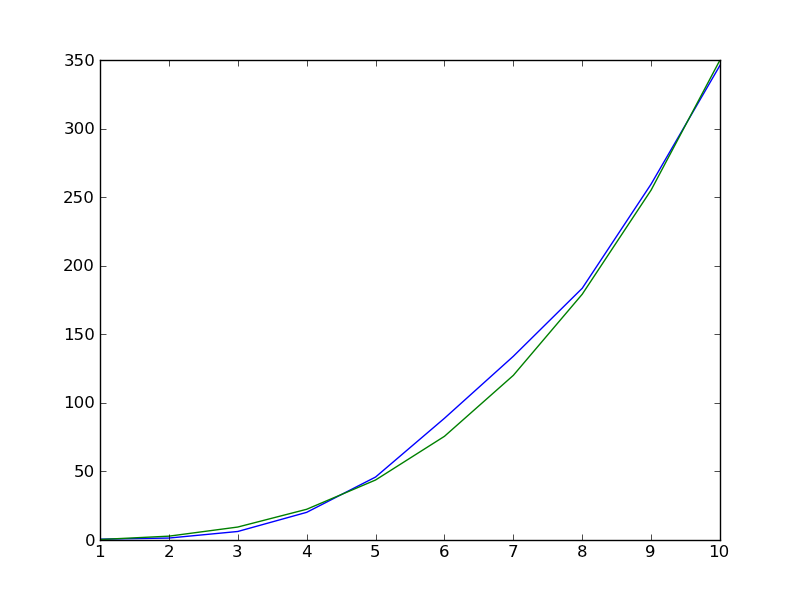
\includegraphics[scale = 0.5]{its_cubic.png}
\caption{Maximum edit distance vs. runtime: actual runtime in blue, cubic curve in green}
\end{center}
\end{figure}

\section{Results}
The algorithm ran in 1817 seconds for the full set of test data, as compared to 11.77 for dnaclust. The frequency culling eliminated 98.4\% of the pairings. We consider this a success for lightly optimized python code, and further improvements could be made by porting the code to cython or C.  
\maketitle

\end{document}
